\documentclass[11pt]{article}

\usepackage[margin=1in]{geometry}
\usepackage[T1]{fontenc}
\usepackage[utf8]{inputenc}
\usepackage{lmodern}
\usepackage{microtype}
\usepackage{amsmath,amssymb,amsthm,mathtools}
\usepackage{bm}
\usepackage{booktabs,array,longtable}
\usepackage{xcolor}
\usepackage[most]{tcolorbox}
\usepackage{tikz}
\usepackage{pgfplots}
\usepackage{pgfplotstable}
\usepackage{enumitem}
\usepackage{caption}
\usepackage{float}
\usepackage{fancyhdr}
\usepackage{titlesec}
\usepackage{hyperref}

\pgfplotsset{compat=1.18}
\usepgfplotslibrary{fillbetween,colormaps,groupplots}
\usetikzlibrary{arrows.meta,calc,positioning,patterns,decorations.pathreplacing,matrix,backgrounds,shapes.geometric}

\hypersetup{colorlinks=true,linkcolor=blue!60!black,urlcolor=blue!60!black,pdftitle={Chapter 26. Multivariable Calculus for Applied Mathematics}}

\setlength{\headheight}{14pt}
\setlength{\parindent}{0pt}
\setlength{\parskip}{0.65em}
\setlist[itemize]{topsep=2pt,itemsep=2pt}
\setlist[enumerate]{topsep=2pt,itemsep=2pt}
\titleformat{\section}{\large\bfseries}{\thesection}{0.6em}{}
\titleformat{\subsection}{\normalsize\bfseries}{\thesubsection}{0.6em}{}

\pagestyle{fancy}
\fancyhf{}
\lhead{Chapter 26. Multivariable Calculus for Applied Mathematics}
\rhead{\thepage}
\renewcommand{\headrulewidth}{0.4pt}

\newtcolorbox{chapterbox}{colback=blue!4,colframe=blue!55!black,boxrule=0.7pt,arc=2mm,left=2mm,right=2mm,top=1mm,bottom=1mm}
\newtcolorbox{goalbox}{colback=green!4,colframe=green!45!black,title=Learning goals,fonttitle=\bfseries,boxrule=0.7pt,arc=2mm}
\newtcolorbox{tipbox}[1][]{colback=green!3,colframe=green!45!black,title=#1,fonttitle=\bfseries,boxrule=0.7pt,arc=2mm}
\newtcolorbox{notebox}[1][]{colback=blue!3,colframe=blue!50!black,title=#1,fonttitle=\bfseries,boxrule=0.7pt,arc=2mm}
\newtcolorbox{importantbox}[1][]{colback=red!3,colframe=red!60!black,title=#1,fonttitle=\bfseries,boxrule=0.7pt,arc=2mm}
\newtcolorbox{warningbox}[1][]{colback=yellow!8,colframe=orange!80!black,title=#1,fonttitle=\bfseries,boxrule=0.7pt,arc=2mm}
\newtcbtheorem[number within=section]{examplebox}{Example}{enhanced,breakable,colback=white,colframe=blue!60!black,colbacktitle=blue!60!black,fonttitle=\bfseries,boxrule=0.7pt,arc=1.5mm,left=2mm,right=2mm,top=1mm,bottom=1mm}{ex}

\newcommand{\R}{\mathbb R}
\newcommand{\grad}{\nabla}
\newcommand{\Div}{\nabla\!\cdot}
\newcommand{\Curl}{\nabla\!\times}
\newcommand{\Lap}{\Delta}
\newcommand{\dd}{\,d}

\begin{document}

\begin{center}
  {\LARGE\bfseries Chapter 26. Multivariable Calculus for Applied Mathematics\par}
  \vspace{0.3em}
  {\large Fields, flows, conservation laws, and numerical models\par}
\end{center}

\begin{chapterbox}
Applied mathematics is the art of turning a real system into a mathematical model, studying the model, computing with it, and interpreting the result. Multivariable calculus is one of the main languages of this process. It tells us how quantities change in space and time, how material flows through regions, how heat diffuses, how forces produce motion, and how energy principles lead to equations.

The previous chapters developed gradients, Jacobians, Hessians, multiple integrals, vector fields, line integrals, surface integrals, and the major integral theorems. This chapter brings those ideas together from an applied mathematics point of view. The goal is not to replace a future course in differential equations, numerical analysis, or partial differential equations. The goal is to show how multivariable calculus becomes the foundation for those subjects.
\end{chapterbox}

In this chapter we study four recurring applied themes:
\begin{enumerate}
  \item \textbf{Local change:} derivatives measure how quantities change at a point.
  \item \textbf{Accumulation:} integrals measure total amount over curves, surfaces, and regions.
  \item \textbf{Balance laws:} divergence and flux express conservation of mass, heat, probability, or charge.
  \item \textbf{Energy principles:} many equations arise by minimizing an energy.
\end{enumerate}

\begin{goalbox}
After completing this chapter, you should be able to:
\begin{itemize}
  \item interpret scalar fields, vector fields, gradient fields, divergence, curl, and the Laplacian in applied models;
  \item derive simple conservation laws from flux balance;
  \item connect the heat equation to diffusion, smoothing, and gradient-based dynamics;
  \item use finite differences to approximate gradients, divergence, and the Laplacian on a grid;
  \item explain how continuous models lead to numerical algorithms;
  \item recognize variational and energy-based formulations;
  \item connect applied calculus ideas to data science, image processing, probability flow, and optimization.
\end{itemize}
\end{goalbox}

\section{The applied mathematics pipeline}

A useful applied mathematics workflow is
\[
\text{system} \longrightarrow \text{variables} \longrightarrow \text{model} \longrightarrow \text{analysis} \longrightarrow \text{computation} \longrightarrow \text{interpretation}.
\]

\begin{figure}[H]
\centering
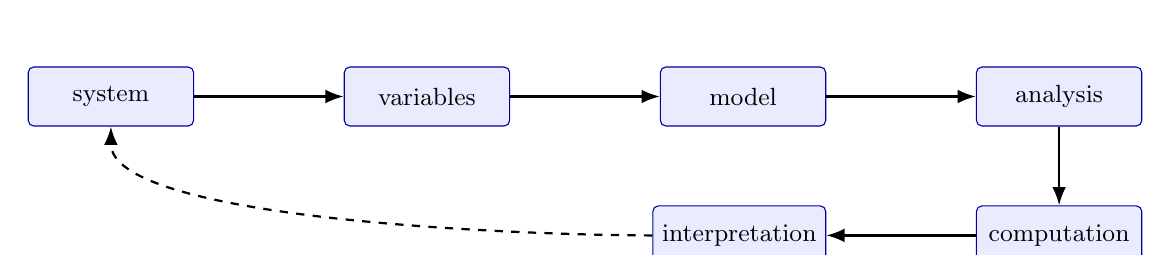
\begin{tikzpicture}[node distance=1.9cm,>=Latex,font=\small]
\tikzstyle{box}=[draw=blue!65!black,fill=blue!8,rounded corners=2pt,minimum width=2.1cm,minimum height=0.75cm,align=center]
\node[box] (sys) {system};
\node[box,right=of sys] (var) {variables};
\node[box,right=of var] (mod) {model};
\node[box,right=of mod] (ana) {analysis};
\node[box,below=1.0cm of ana] (comp) {computation};
\node[box,left=of comp] (interp) {interpretation};
\draw[->,thick] (sys)--(var);
\draw[->,thick] (var)--(mod);
\draw[->,thick] (mod)--(ana);
\draw[->,thick] (ana)--(comp);
\draw[->,thick] (comp)--(interp);
\draw[->,thick,dashed] (interp.west) .. controls +(left:1.5cm) and +(down:1.2cm) .. (sys.south);
\end{tikzpicture}
\caption{The applied mathematics pipeline. Interpretation often feeds back into the choice of variables and model.}
\end{figure}

For example, if $u(x,t)$ is the temperature of a thin rod at position $x$ and time $t$, a physical law says heat flows from hot regions to cold regions. A calculus model converts this statement into a differential equation. A numerical method approximates the equation on a finite grid, and a simulation helps us understand the temperature evolution.

\begin{center}
\begin{tabular}{@{}lll@{}}
\toprule
Applied setting & Typical field & Calculus object \\
\midrule
heat flow & $u(x,y,t)$ & scalar field \\
fluid velocity & $F(x,y,z,t)$ & vector field \\
probability density & $p(x,t)$ & scalar field with integral $1$ \\
image intensity & $I(x,y)$ & scalar field on a pixel grid \\
model loss & $L(\theta)$ & scalar field on parameter space \\
gradient descent & $\theta'(t)=-\grad L(\theta)$ & vector field on parameter space \\
\bottomrule
\end{tabular}
\end{center}

A key message of this chapter is that the same calculus operators appear across many disciplines.

\section{Scalar fields, vector fields, and operators}

A scalar field assigns a number to each point. Examples include temperature, pressure, density, altitude, potential energy, image brightness, or a loss function:
\[
u=u(x,y,z).
\]
A vector field assigns a vector to each point. Examples include velocity, force, heat flux, electric field, gradient direction, or parameter update direction:
\[
F(x,y,z)=\langle P(x,y,z),Q(x,y,z),R(x,y,z)\rangle.
\]

The most important differential operators in applied mathematics are
\[
\grad u=\left\langle u_x,u_y,u_z\right\rangle,
\qquad
\Div F=P_x+Q_y+R_z,
\]
\[
\Curl F=\left\langle R_y-Q_z,\; P_z-R_x,\; Q_x-P_y\right\rangle,
\qquad
\Lap u=\Div(\grad u)=u_{xx}+u_{yy}+u_{zz}.
\]
The operator $\Lap$ is called the \emph{Laplacian}. It is one of the central operators in applied mathematics.

\begin{tipbox}[Interpretation of the operators]
\begin{itemize}
  \item $\grad u$ points in the direction of fastest increase of $u$.
  \item $\Div F$ measures local expansion or compression of a vector field.
  \item $\Curl F$ measures local rotation.
  \item $\Lap u$ compares a value with nearby values and measures local curvature or imbalance.
\end{itemize}
\end{tipbox}

\begin{examplebox}{Gradient, divergence, curl, and Laplacian}{operators}
Let $u(x,y,z)=x^2+y^2+z^2$. Then
\[
\grad u=\langle 2x,2y,2z\rangle,
\qquad
\Lap u=u_{xx}+u_{yy}+u_{zz}=2+2+2=6.
\]
If $F(x,y,z)=\langle x,y,z\rangle$, then
\[
\Div F=1+1+1=3,
\qquad
\Curl F=\langle 0,0,0\rangle.
\]
This vector field expands outward from the origin but does not rotate.
\end{examplebox}

\begin{figure}[H]
\centering
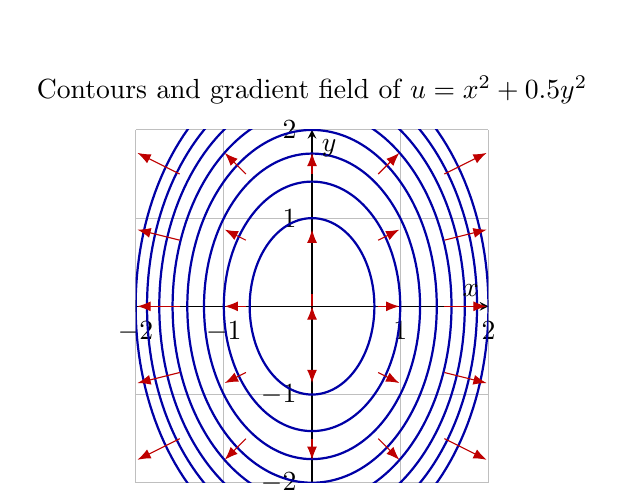
\begin{tikzpicture}
\begin{axis}[
  width=0.66\textwidth,height=0.5\textwidth,
  xmin=-2,xmax=2,ymin=-2,ymax=2,
  axis equal image,axis lines=middle,
  xlabel={$x$},ylabel={$y$},grid=both,
  title={Contours and gradient field of $u=x^2+0.5y^2$}
]
\foreach \c in {0.5,1,1.5,2,2.5,3,3.5,4}{
  \addplot[blue!65!black,thick,domain=0:360,samples=180] ({sqrt(\c)*cos(x)},{sqrt(2*\c)*sin(x)});
}
\foreach \a in {-1.5,-0.75,0,0.75,1.5}{
  \foreach \b in {-1.5,-0.75,0,0.75,1.5}{
    \pgfmathsetmacro{\aa}{\a+0.16*(2*\a)}
    \pgfmathsetmacro{\bb}{\b+0.16*(\b)}
    \addplot[red!75!black,-Latex] coordinates {(\a,\b) (\aa,\bb)};
  }
}
\end{axis}
\end{tikzpicture}
\caption{A scalar field, its contours, and its gradient vectors. The gradient points uphill and is perpendicular to level curves.}
\end{figure}

\section{Balance laws and conservation}

Many applied models begin with a balance principle:
\[
\text{rate of change inside a region}=\text{inflow}-\text{outflow}+\text{sources}.
\]
Suppose $\rho(x,y,z,t)$ is the density of a quantity and $J(x,y,z,t)$ is its flux field. For a fixed region $E$, the total amount inside $E$ is
\[
\int_E \rho\,dV.
\]
The outward flux through the boundary $\partial E$ is
\[
\iint_{\partial E}J\cdot n\,dS.
\]
If there are no internal sources, conservation says
\[
\frac{d}{dt}\int_E \rho\,dV=-\iint_{\partial E}J\cdot n\,dS.
\]
Using the Divergence Theorem,
\[
\iint_{\partial E}J\cdot n\,dS=\int_E \Div J\,dV.
\]
Therefore
\[
\int_E \rho_t\,dV=-\int_E \Div J\,dV.
\]
Since this should hold for every region $E$, the local form is
\[
\rho_t+\Div J=0.
\]
This is called a \emph{continuity equation}.

\begin{importantbox}[Conservation law template]
A large class of applied models has the form
\[
\rho_t+\Div J=s,
\]
where $\rho$ is a density, $J$ is a flux, and $s$ is a source term.
\end{importantbox}

\begin{examplebox}{Source, sink, and incompressible fields}{sourcesink}
In the plane, consider
\[
F_1(x,y)=\langle x,y\rangle,\qquad F_2(x,y)=\langle -x,-y\rangle,\qquad F_3(x,y)=\langle -y,x\rangle.
\]
Their divergences are
\[
\Div F_1=2,\qquad \Div F_2=-2,\qquad \Div F_3=0.
\]
The first field is a source, the second is a sink, and the third is rotation without local expansion.
\end{examplebox}

\begin{figure}[H]
\centering
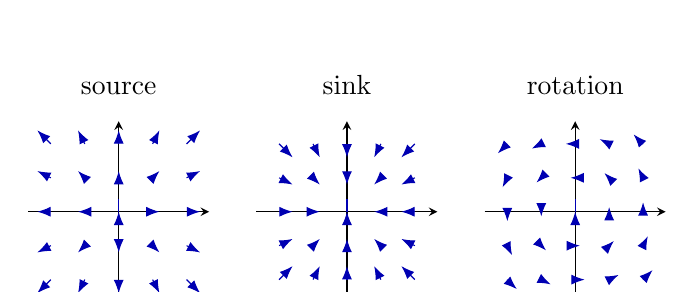
\begin{tikzpicture}
\begin{groupplot}[
  group style={group size=3 by 1,horizontal sep=0.6cm},
  width=0.32\textwidth,height=0.32\textwidth,
  xmin=-2,xmax=2,ymin=-2,ymax=2,
  axis equal image,axis lines=middle,xtick=\empty,ytick=\empty
]
\nextgroupplot[title={source}]
\foreach \a in {-1.5,-0.75,0,0.75,1.5}{\foreach \b in {-1.5,-0.75,0,0.75,1.5}{\pgfmathsetmacro{\aa}{\a+0.2*\a}\pgfmathsetmacro{\bb}{\b+0.2*\b}\addplot[blue!70!black,-Latex] coordinates {(\a,\b) (\aa,\bb)};}}
\nextgroupplot[title={sink}]
\foreach \a in {-1.5,-0.75,0,0.75,1.5}{\foreach \b in {-1.5,-0.75,0,0.75,1.5}{\pgfmathsetmacro{\aa}{\a-0.2*\a}\pgfmathsetmacro{\bb}{\b-0.2*\b}\addplot[blue!70!black,-Latex] coordinates {(\a,\b) (\aa,\bb)};}}
\nextgroupplot[title={rotation}]
\foreach \a in {-1.5,-0.75,0,0.75,1.5}{\foreach \b in {-1.5,-0.75,0,0.75,1.5}{\pgfmathsetmacro{\aa}{\a-0.14*\b}\pgfmathsetmacro{\bb}{\b+0.14*\a}\addplot[blue!70!black,-Latex] coordinates {(\a,\b) (\aa,\bb)};}}
\end{groupplot}
\end{tikzpicture}
\caption{Three basic vector fields: source, sink, and rotational field. Divergence distinguishes expansion from compression.}
\end{figure}

\section{Diffusion and the heat equation}

One of the most important applied models is the heat equation. Suppose $u(x,t)$ is temperature along a rod. Heat flows from high temperature to low temperature. A common model for heat flux is Fourier's law:
\[
J=-k\grad u,
\]
where $k>0$ is the conductivity. The minus sign means heat flows downhill, opposite the direction of increasing temperature.

If heat is conserved and $J=-k\grad u$, then
\[
u_t+\Div J=0.
\]
Substituting the flux law gives
\[
u_t-k\Div(\grad u)=0,
\]
so
\[
u_t=k\Lap u.
\]
This is the \emph{heat equation}. In one spatial dimension, $u_t=ku_{xx}$. In two spatial dimensions, $u_t=k(u_{xx}+u_{yy})$.

\begin{notebox}[Why the Laplacian appears]
The Laplacian measures whether a point is higher or lower than its neighbors. If a point is hotter than its neighbors, heat diffuses away. If it is colder than its neighbors, heat diffuses in. This local averaging behavior is exactly what the heat equation models.
\end{notebox}

\begin{figure}[H]
\centering
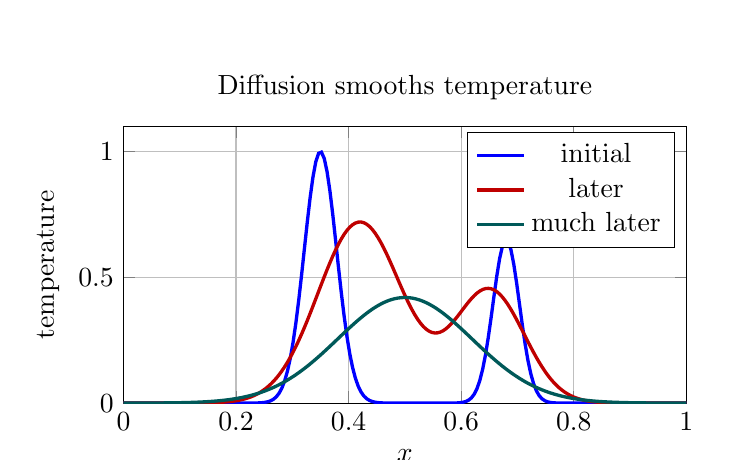
\begin{tikzpicture}
\begin{axis}[
  width=0.72\textwidth,height=0.42\textwidth,
  xmin=0,xmax=1,ymin=0,ymax=1.1,
  xlabel={$x$},ylabel={temperature},grid=both,
  title={Diffusion smooths temperature},
  legend style={at={(0.98,0.98)},anchor=north east,fill=white}
]
\addplot[very thick,blue,domain=0:1,samples=200] {exp(-600*(x-0.35)^2)+0.65*exp(-900*(x-0.68)^2)};\addlegendentry{initial}
\addplot[very thick,red!75!black,domain=0:1,samples=200] {0.72*exp(-90*(x-0.42)^2)+0.45*exp(-130*(x-0.65)^2)};\addlegendentry{later}
\addplot[very thick,teal!70!black,domain=0:1,samples=200] {0.42*exp(-35*(x-0.5)^2)};\addlegendentry{much later}
\end{axis}
\end{tikzpicture}
\caption{A localized temperature profile spreads and smooths over time, as predicted by the one-dimensional heat equation.}
\end{figure}

\section{The Laplacian as local averaging}

On a grid, the two-dimensional Laplacian is often approximated by
\[
\Lap u(x_i,y_j)\approx \frac{u_{i+1,j}+u_{i-1,j}+u_{i,j+1}+u_{i,j-1}-4u_{i,j}}{h^2}.
\]
This formula compares a grid value to its four nearest neighbors. It appears in numerical partial differential equations, image processing, graph learning, and spatial statistics.

\begin{figure}[H]
\centering
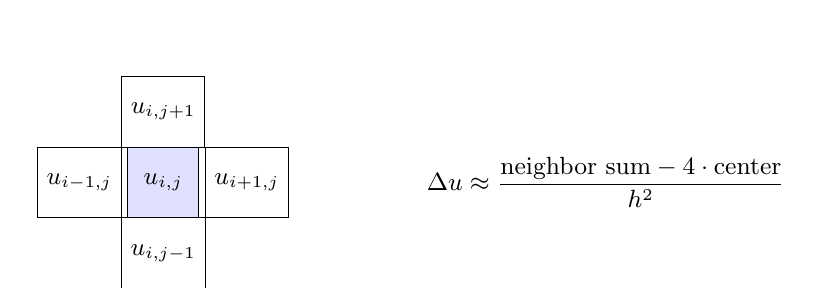
\begin{tikzpicture}[font=\small]
\matrix[matrix of nodes,nodes={draw,minimum size=0.9cm,anchor=center},column sep=-\pgflinewidth,row sep=-\pgflinewidth] (m) {
 & $u_{i,j+1}$ & \\
$u_{i-1,j}$ & |[fill=blue!12]|$u_{i,j}$ & $u_{i+1,j}$ \\
 & $u_{i,j-1}$ & \\
};
\node[right=1.5cm of m] {$\displaystyle \Lap u\approx\frac{\text{neighbor sum}-4\cdot\text{center}}{h^2}$};
\end{tikzpicture}
\caption{The five-point stencil for the two-dimensional discrete Laplacian.}
\end{figure}

\section{Advection and transport}

Diffusion describes spreading. Advection describes transport by a velocity field. Suppose $\rho(x,y,t)$ is the density of a substance moving with velocity field
\[
v(x,y)=\langle P(x,y),Q(x,y)\rangle.
\]
The flux is $J=\rho v$, and the conservation law becomes
\[
\rho_t+\Div(\rho v)=0.
\]
If the velocity field is incompressible, meaning $\Div v=0$, then
\[
\rho_t+v\cdot\grad \rho=0.
\]
The term $v\cdot\grad\rho$ is a directional derivative: it measures how density changes in the direction of the flow.

\begin{examplebox}{Rotation transports density}{rotation}
For $v(x,y)=\langle -y,x\rangle$, particles rotate around the origin. Since
\[
\Div v=\frac{\partial(-y)}{\partial x}+\frac{\partial x}{\partial y}=0,
\]
this field preserves area locally.
\end{examplebox}

\begin{figure}[H]
\centering
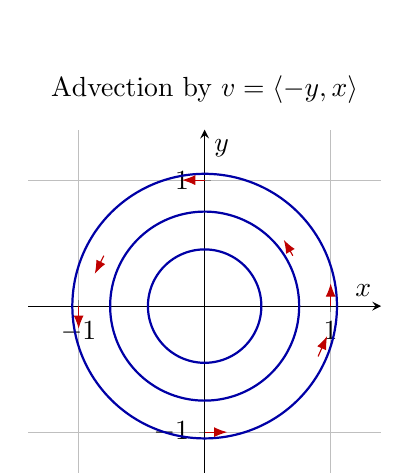
\begin{tikzpicture}
\begin{axis}[
  width=0.5\textwidth,height=0.5\textwidth,
  xmin=-1.4,xmax=1.4,ymin=-1.4,ymax=1.4,
  axis equal image,axis lines=middle,xlabel={$x$},ylabel={$y$},grid=both,
  title={Advection by $v=\langle -y,x\rangle$}
]
\foreach \r in {0.45,0.75,1.05}{\addplot[blue!65!black,thick,domain=0:360,samples=180] ({\r*cos(x)},{\r*sin(x)});}
\foreach \a/\b in {1/0,0.7/0.4,0/1,-0.8/0.4,-1/0,0/-1,0.9/-0.4}{
  \pgfmathsetmacro{\aa}{\a-0.18*\b}
  \pgfmathsetmacro{\bb}{\b+0.18*\a}
  \addplot[red!75!black,-Latex] coordinates {(\a,\b) (\aa,\bb)};
}
\end{axis}
\end{tikzpicture}
\caption{Particle trajectories in a rotational velocity field. Advection transports quantities along flow lines.}
\end{figure}

\section{Steady states and Laplace's equation}

A steady state is a solution that does not change with time. For the heat equation $u_t=k\Lap u$, a steady state satisfies
\[
\Lap u=0.
\]
This is \emph{Laplace's equation}. Functions satisfying $\Lap u=0$ are called \emph{harmonic functions}. Laplace's equation appears in heat conduction, electrostatics, gravitational potential, fluid flow, and image interpolation.

\begin{examplebox}{A harmonic function}{harmonic}
Let $u(x,y)=x^2-y^2$. Then $u_{xx}=2$ and $u_{yy}=-2$, so
\[
\Lap u=u_{xx}+u_{yy}=0.
\]
Thus $u(x,y)=x^2-y^2$ is harmonic.
\end{examplebox}

\begin{figure}[H]
\centering
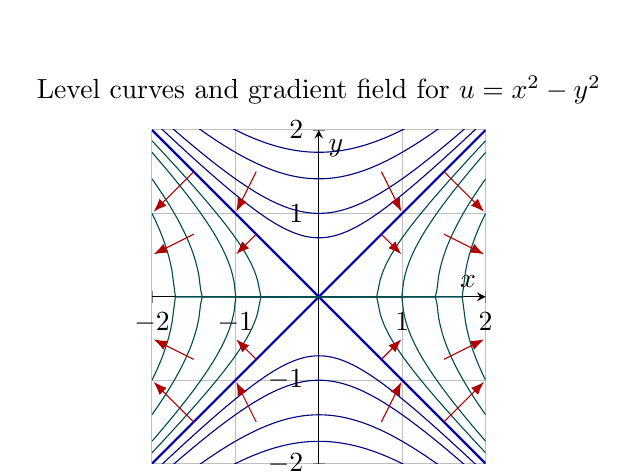
\begin{tikzpicture}
\begin{axis}[
  width=0.66\textwidth,height=0.48\textwidth,
  xmin=-2,xmax=2,ymin=-2,ymax=2,
  axis equal image,axis lines=middle,xlabel={$x$},ylabel={$y$},grid=both,
  title={Level curves and gradient field for $u=x^2-y^2$}
]
\addplot[domain=-2:2,samples=200,blue!70!black,thick] {x};
\addplot[domain=-2:2,samples=200,blue!70!black,thick] {-x};
\foreach \c in {0.5,1,2,3}{
  \addplot[domain=-2:2,samples=200,blue!50!black] {sqrt(x^2+\c)};
  \addplot[domain=-2:2,samples=200,blue!50!black] {-sqrt(x^2+\c)};
  \addplot[domain=-2:2,samples=200,teal!60!black] {sqrt(max(0,x^2-\c))};
  \addplot[domain=-2:2,samples=200,teal!60!black] {-sqrt(max(0,x^2-\c))};
}
\foreach \a in {-1.5,-0.75,0.75,1.5}{\foreach \b in {-1.5,-0.75,0.75,1.5}{\pgfmathsetmacro{\aa}{\a+0.16*(2*\a)}\pgfmathsetmacro{\bb}{\b+0.16*(-2*\b)}\addplot[red!70!black,-Latex] coordinates {(\a,\b) (\aa,\bb)};}}
\end{axis}
\end{tikzpicture}
\caption{The harmonic function $u=x^2-y^2$ has zero Laplacian. It bends upward in one direction and downward in the other.}
\end{figure}

\section{Numerical derivatives on grids}

In applied mathematics, functions are often known only through sampled values. For grid spacing $h$, common finite-difference approximations are
\[
u_x(x_i,y_j)\approx \frac{u_{i+1,j}-u_{i-1,j}}{2h},
\qquad
u_y(x_i,y_j)\approx \frac{u_{i,j+1}-u_{i,j-1}}{2h},
\]
\[
\Lap u(x_i,y_j)\approx \frac{u_{i+1,j}+u_{i-1,j}+u_{i,j+1}+u_{i,j-1}-4u_{i,j}}{h^2}.
\]
These approximations convert calculus into linear algebra. A differential operator becomes a matrix or a stencil.

\begin{tipbox}[Continuous-discrete dictionary]
\begin{center}
\begin{tabular}{@{}ll@{}}
\toprule
Continuous calculus & Discrete computation \\
\midrule
function $u(x,y)$ & array of values \\
derivative $u_x$ & finite difference \\
gradient $\grad u$ & pair of arrays \\
Laplacian $\Lap u$ & stencil or sparse matrix \\
integral & sum times area element \\
partial differential equation & update rule or linear system \\
\bottomrule
\end{tabular}
\end{center}
\end{tipbox}

\section{Variational principles and energy minimization}

Many equations in applied mathematics come from minimizing an energy. A simple example is the Dirichlet energy
\[
E[u]=\frac12\int_D |\grad u|^2\,dA.
\]
A function that minimizes this energy subject to fixed boundary values satisfies Laplace's equation
\[
\Lap u=0
\]
inside the domain.

The intuition is that minimizing $\int |\grad u|^2$ favors smooth functions. The minimizer is as smooth as possible while still matching boundary constraints. This idea appears in elastic membranes, electrostatic potentials, image denoising and interpolation, smoothing splines, graph-based semi-supervised learning, and regularization in inverse problems.

\begin{examplebox}{Smoothing by energy minimization}{smoothing}
Suppose we observe noisy data $y_i$ and want a smooth curve $u_i$. A discrete energy is
\[
E(u)=\sum_i(u_i-y_i)^2+\lambda\sum_i(u_{i+1}-u_i)^2.
\]
The first term keeps $u$ close to the data. The second term penalizes roughness. The parameter $\lambda$ controls the tradeoff.
\end{examplebox}

\begin{figure}[H]
\centering
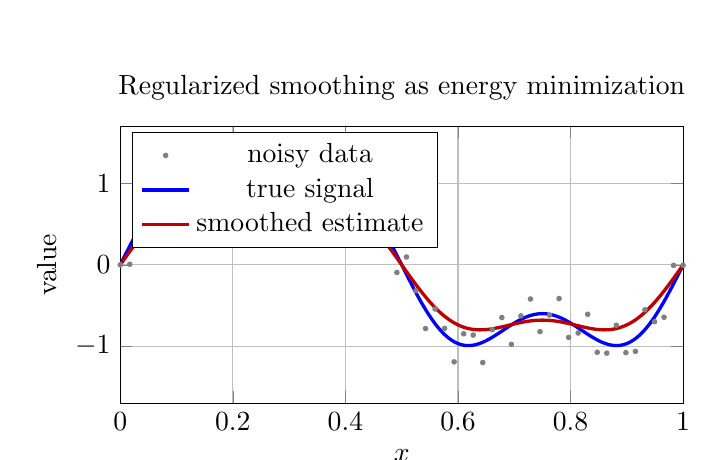
\begin{tikzpicture}
\begin{axis}[
  width=0.72\textwidth,height=0.42\textwidth,
  xmin=0,xmax=1,ymin=-1.7,ymax=1.7,
  xlabel={$x$},ylabel={value},grid=both,
  title={Regularized smoothing as energy minimization},
  legend style={at={(0.02,0.98)},anchor=north west,fill=white}
]
\addplot[only marks,mark=*,mark size=0.8pt,gray,domain=0:1,samples=60] {sin(deg(2*pi*x))+0.4*sin(deg(6*pi*x))+0.25*sin(deg(80*pi*x))};\addlegendentry{noisy data}
\addplot[very thick,blue,domain=0:1,samples=200] {sin(deg(2*pi*x))+0.4*sin(deg(6*pi*x))};\addlegendentry{true signal}
\addplot[very thick,red!75!black,domain=0:1,samples=200] {0.9*sin(deg(2*pi*x))+0.22*sin(deg(6*pi*x))};\addlegendentry{smoothed estimate}
\end{axis}
\end{tikzpicture}
\caption{Energy-based smoothing balances fidelity to noisy data with a penalty on roughness.}
\end{figure}

\section{Gradient flows}

Optimization can also be viewed as an applied dynamical system. Given an energy or loss function $E(x)$, gradient flow is the differential equation
\[
\frac{dx}{dt}=-\grad E(x).
\]
This equation moves downhill as quickly as possible in continuous time. Gradient descent is a discrete approximation:
\[
x_{k+1}=x_k-\eta\grad E(x_k).
\]
Thus optimization algorithms are closely related to differential equations.

\begin{examplebox}{Gradient flow toward a minimum}{gradflow}
For an energy landscape $E(x,y)$, gradient flow follows the vector field $-\grad E$. The motion crosses contours in the downhill direction and tends to move toward local minima.
\end{examplebox}

\begin{figure}[H]
\centering
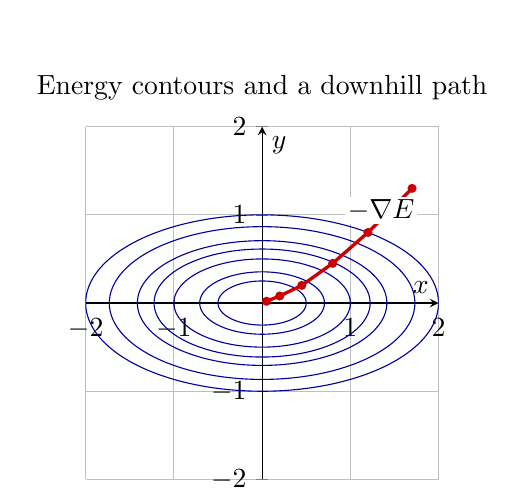
\begin{tikzpicture}
\begin{axis}[
  width=0.58\textwidth,height=0.5\textwidth,
  xmin=-2,xmax=2,ymin=-2,ymax=2,
  axis equal image,axis lines=middle,xlabel={$x$},ylabel={$y$},grid=both,
  title={Energy contours and a downhill path}
]
\foreach \c in {0.25,0.5,1,1.5,2,3,4}{\addplot[domain=0:360,samples=180,blue!60!black] ({sqrt(\c)*cos(x)},{0.5*sqrt(\c)*sin(x)});}
\addplot[red!80!black,very thick,mark=*,mark size=1pt] coordinates {(1.7,1.3) (1.2,0.8) (0.8,0.45) (0.45,0.2) (0.2,0.08) (0.05,0.02)};
\node[fill=white,inner sep=1pt] at (axis cs:1.35,1.05) {$-\grad E$};
\end{axis}
\end{tikzpicture}
\caption{Gradient flow follows the vector field $-\grad E$ and moves downhill on an energy landscape.}
\end{figure}

\section{From continuous models to numerical algorithms}

Applied mathematics often converts a continuous model into a finite-dimensional computation. The common steps are:
\begin{enumerate}
  \item Choose variables. Decide what the unknown function represents.
  \item State a law. Use balance, geometry, probability, or energy.
  \item Write equations. Express the law using derivatives and integrals.
  \item Choose boundary and initial conditions. Models need enough information to determine a solution.
  \item Discretize. Replace derivatives by finite differences, finite elements, or spectral approximations.
  \item Compute. Solve a system of algebraic equations or run an update rule.
  \item Validate. Compare against data, units, limiting cases, or known solutions.
\end{enumerate}

For the one-dimensional heat equation $u_t=ku_{xx}$, a simple explicit method is
\[
u_i^{n+1}=u_i^n+r(u_{i+1}^n-2u_i^n+u_{i-1}^n),
\qquad
r=\frac{k\Delta t}{(\Delta x)^2}.
\]
This formula says: update each value using the difference between the value and its neighbors.

\begin{warningbox}[Stability matters]
A numerical formula can be mathematically reasonable but computationally unstable. For the explicit heat equation scheme, the time step must be sufficiently small relative to the spatial grid size. This is a first glimpse of numerical analysis.
\end{warningbox}

\section{Applied mathematics examples}

\subsection*{Image denoising}
An image can be viewed as a scalar field $I(x,y)$. Diffusion smooths the image by reducing sharp local variations. A simple denoising model is $I_t=\Lap I$. This smooths noise but may also blur edges. More advanced models modify the diffusion coefficient so smoothing happens more strongly in flat regions and less strongly near edges.

\subsection*{Probability diffusion}
A probability density $p(x,t)$ can evolve by diffusion:
\[
p_t=Dp_{xx}.
\]
Under appropriate boundary conditions this equation preserves total probability:
\[
\int p(x,t)\,dx=1.
\]
This connects calculus to stochastic processes, Brownian motion, and statistical physics.

\subsection*{Inverse problems}
In an inverse problem, we infer hidden causes from observed effects. A common regularized model minimizes
\[
\|Au-y\|^2+\lambda\|Lu\|^2,
\]
where $A$ models the measurement process, $y$ is observed data, and $L$ measures roughness.

\subsection*{Conservation in networks}
Even when a system is not spatially continuous, conservation ideas remain. In a network, mass or probability may flow along edges. The graph divergence at a node measures net outflow. The graph Laplacian plays the role of the continuous Laplacian. This is why Laplacian ideas appear in spectral clustering, graph signal processing, semi-supervised learning, and diffusion maps.

\begin{figure}[H]
\centering
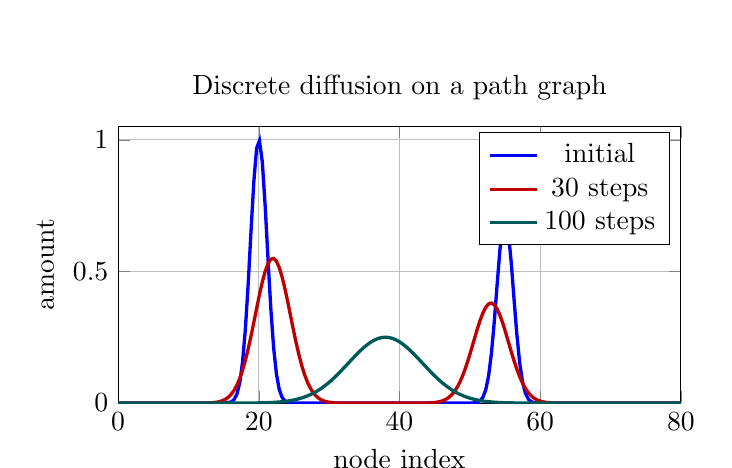
\begin{tikzpicture}
\begin{axis}[
  width=0.72\textwidth,height=0.42\textwidth,
  xmin=0,xmax=80,ymin=0,ymax=1.05,
  xlabel={node index},ylabel={amount},grid=both,
  title={Discrete diffusion on a path graph},
  legend style={at={(0.98,0.98)},anchor=north east,fill=white}
]
\addplot[very thick,blue,domain=0:80,samples=200] {exp(-0.35*(x-20)^2)+0.7*exp(-0.35*(x-55)^2)};\addlegendentry{initial}
\addplot[very thick,red!75!black,domain=0:80,samples=200] {0.55*exp(-0.08*(x-22)^2)+0.38*exp(-0.08*(x-53)^2)};\addlegendentry{30 steps}
\addplot[very thick,teal!70!black,domain=0:80,samples=200] {0.25*exp(-0.018*(x-38)^2)};\addlegendentry{100 steps}
\end{axis}
\end{tikzpicture}
\caption{Discrete diffusion on a one-dimensional network. Repeated averaging behaves like a graph version of the heat equation.}
\end{figure}

\section{Common modeling mistakes}

Applied mathematics is powerful, but models require judgment. Common mistakes include:
\begin{itemize}
  \item confusing density with total amount;
  \item forgetting units when defining flux or source terms;
  \item using a local equation without appropriate boundary conditions;
  \item assuming a numerical solution is accurate without checking stability or convergence;
  \item treating a model as reality rather than as a simplified representation;
  \item ignoring whether a vector field is conservative, divergence-free, or rotational;
  \item applying a theorem without checking orientation, smoothness, or region assumptions.
\end{itemize}
A good model should be mathematically consistent, computationally feasible, and interpretable in context.

\section{Computational lab: finite differences and diffusion}

The following functions form a small numerical calculus toolkit for scalar fields on a grid:
\begin{verbatim}
def central_gradient(U, h):
    Ux[:,1:-1] = (U[:,2:] - U[:,:-2])/(2*h)
    Uy[1:-1,:] = (U[2:,:] - U[:-2,:])/(2*h)
    return Ux, Uy

def five_point_laplacian(U, h):
    Lap[1:-1,1:-1] = (
        U[2:,1:-1] + U[:-2,1:-1]
        + U[1:-1,2:] + U[1:-1,:-2]
        - 4*U[1:-1,1:-1]
    )/(h**2)
    return Lap
\end{verbatim}
For $u(x,y)=x^2+y^2$, the exact value is $\Lap u=4$. The numerical value should be close to $4$ on interior grid points.

\section{Chapter summary}

This chapter connected multivariable calculus to applied mathematics. The central ideas are:
\begin{itemize}
  \item scalar fields describe quantities such as temperature, density, potential, image intensity, and loss;
  \item vector fields describe forces, velocities, fluxes, and gradient flows;
  \item conservation laws combine time derivatives with flux integrals;
  \item the Divergence Theorem converts global flux balance into local differential equations;
  \item diffusion and the heat equation arise from conservation plus a flux law;
  \item the Laplacian measures local imbalance and acts like a continuous averaging operator;
  \item finite differences turn derivatives into computational formulas;
  \item energy minimization leads to differential equations and regularized algorithms;
  \item gradient flow connects optimization with dynamical systems.
\end{itemize}
The main conceptual bridge is
\[
\text{calculus operators}\longrightarrow \text{models}\longrightarrow \text{algorithms}.
\]

\section{Exercises}

\subsection*{Conceptual exercises}
\begin{enumerate}
  \item Explain the difference between a scalar field and a vector field. Give two examples of each from applied mathematics.
  \item What does $\grad u$ measure? Why is it perpendicular to level curves?
  \item What does $\Div F$ measure physically?
  \item What does $\Lap u$ measure intuitively?
  \item Explain why heat should flow in the direction $-\grad u$ rather than $\grad u$.
  \item What is the difference between diffusion and advection?
  \item Why does a conservation law naturally involve flux through the boundary of a region?
  \item Explain why a steady-state heat equation leads to $\Lap u=0$.
  \item Why do numerical models require boundary conditions?
  \item Explain the connection between gradient descent and gradient flow.
\end{enumerate}

\subsection*{Computational exercises}
\begin{enumerate}[start=11]
  \item For $u(x,y)=e^{-x^2-y^2}$, compute $\grad u$ and $\Lap u$.
  \item For $F(x,y)=\langle x^2,xy\rangle$, compute $\Div F$ and interpret the result.
  \item For $F(x,y)=\langle -y,x\rangle$, compute divergence and curl.
  \item Use finite differences to approximate $u_x$ and $u_y$ for $u(x,y)=\sin x\cos y$ on a grid.
  \item Use the five-point stencil to approximate $\Lap u$ for $u(x,y)=x^2+y^2$.
  \item Simulate one-dimensional diffusion with a different initial condition.
  \item Simulate two-dimensional diffusion from a square-shaped hot region.
  \item Compare numerical diffusion using two different time step sizes.
  \item Implement gradient descent for $E(x,y)=x^2+4y^2$ and plot the path.
  \item Solve a smoothing problem using $E(u)=\sum_i(u_i-y_i)^2+\lambda\sum_i(u_{i+1}-u_i)^2$ for several values of $\lambda$.
\end{enumerate}

\subsection*{Applied exercises}
\begin{enumerate}[start=21]
  \item Derive the heat equation from $\rho_t+\Div J=0$ and Fourier's law $J=-k\grad u$.
  \item Suppose $p(x,t)$ is a probability density satisfying $p_t=Dp_{xx}$ on a closed interval with no-flux boundary conditions. Explain why total probability is conserved.
  \item A pollutant concentration $c(x,y,t)$ moves with velocity $v(x,y)$ and diffuses with coefficient $D$. Explain the model $c_t+v\cdot\grad c=D\Lap c$ term by term.
  \item In image processing, why might ordinary diffusion blur edges? How might one modify the model to reduce edge blurring?
  \item In a loss landscape $L(\theta)$, explain the difference between gradient flow and Newton's method.
\end{enumerate}

\subsection*{Challenge exercises}
\begin{enumerate}[start=26]
  \item Let $u(x,y)=\log\sqrt{x^2+y^2}$ for $(x,y)\ne(0,0)$. Show that $\Lap u=0$ away from the origin.
  \item Let $F=\grad u$. Show that $\Div F=\Lap u$.
  \item Let $v(x,y)=\langle -y,x\rangle$. Show that the flow preserves $x^2+y^2$.
  \item Derive the finite-difference update $u_i^{n+1}=u_i^n+r(u_{i+1}^n-2u_i^n+u_{i-1}^n)$ from $u_t=ku_{xx}$.
  \item For $E(u)=\|u-y\|^2+\lambda\|Du\|^2$, show that the minimizer satisfies $(I+\lambda D^TD)u=y$.
\end{enumerate}

\end{document}
